\documentclass[]{article}
\usepackage{lmodern}
\usepackage{amssymb,amsmath}
\usepackage{ifxetex,ifluatex}
\usepackage{fixltx2e} % provides \textsubscript
\ifnum 0\ifxetex 1\fi\ifluatex 1\fi=0 % if pdftex
  \usepackage[T1]{fontenc}
  \usepackage[utf8]{inputenc}
\else % if luatex or xelatex
  \ifxetex
    \usepackage{mathspec}
  \else
    \usepackage{fontspec}
  \fi
  \defaultfontfeatures{Ligatures=TeX,Scale=MatchLowercase}
\fi
% use upquote if available, for straight quotes in verbatim environments
\IfFileExists{upquote.sty}{\usepackage{upquote}}{}
% use microtype if available
\IfFileExists{microtype.sty}{%
\usepackage{microtype}
\UseMicrotypeSet[protrusion]{basicmath} % disable protrusion for tt fonts
}{}
\usepackage[margin=1in]{geometry}
\usepackage{hyperref}
\hypersetup{unicode=true,
            pdftitle={DATA 605 - Final Exam},
            pdfauthor={Omer Ozeren},
            pdfborder={0 0 0},
            breaklinks=true}
\urlstyle{same}  % don't use monospace font for urls
\usepackage{color}
\usepackage{fancyvrb}
\newcommand{\VerbBar}{|}
\newcommand{\VERB}{\Verb[commandchars=\\\{\}]}
\DefineVerbatimEnvironment{Highlighting}{Verbatim}{commandchars=\\\{\}}
% Add ',fontsize=\small' for more characters per line
\usepackage{framed}
\definecolor{shadecolor}{RGB}{248,248,248}
\newenvironment{Shaded}{\begin{snugshade}}{\end{snugshade}}
\newcommand{\KeywordTok}[1]{\textcolor[rgb]{0.13,0.29,0.53}{\textbf{#1}}}
\newcommand{\DataTypeTok}[1]{\textcolor[rgb]{0.13,0.29,0.53}{#1}}
\newcommand{\DecValTok}[1]{\textcolor[rgb]{0.00,0.00,0.81}{#1}}
\newcommand{\BaseNTok}[1]{\textcolor[rgb]{0.00,0.00,0.81}{#1}}
\newcommand{\FloatTok}[1]{\textcolor[rgb]{0.00,0.00,0.81}{#1}}
\newcommand{\ConstantTok}[1]{\textcolor[rgb]{0.00,0.00,0.00}{#1}}
\newcommand{\CharTok}[1]{\textcolor[rgb]{0.31,0.60,0.02}{#1}}
\newcommand{\SpecialCharTok}[1]{\textcolor[rgb]{0.00,0.00,0.00}{#1}}
\newcommand{\StringTok}[1]{\textcolor[rgb]{0.31,0.60,0.02}{#1}}
\newcommand{\VerbatimStringTok}[1]{\textcolor[rgb]{0.31,0.60,0.02}{#1}}
\newcommand{\SpecialStringTok}[1]{\textcolor[rgb]{0.31,0.60,0.02}{#1}}
\newcommand{\ImportTok}[1]{#1}
\newcommand{\CommentTok}[1]{\textcolor[rgb]{0.56,0.35,0.01}{\textit{#1}}}
\newcommand{\DocumentationTok}[1]{\textcolor[rgb]{0.56,0.35,0.01}{\textbf{\textit{#1}}}}
\newcommand{\AnnotationTok}[1]{\textcolor[rgb]{0.56,0.35,0.01}{\textbf{\textit{#1}}}}
\newcommand{\CommentVarTok}[1]{\textcolor[rgb]{0.56,0.35,0.01}{\textbf{\textit{#1}}}}
\newcommand{\OtherTok}[1]{\textcolor[rgb]{0.56,0.35,0.01}{#1}}
\newcommand{\FunctionTok}[1]{\textcolor[rgb]{0.00,0.00,0.00}{#1}}
\newcommand{\VariableTok}[1]{\textcolor[rgb]{0.00,0.00,0.00}{#1}}
\newcommand{\ControlFlowTok}[1]{\textcolor[rgb]{0.13,0.29,0.53}{\textbf{#1}}}
\newcommand{\OperatorTok}[1]{\textcolor[rgb]{0.81,0.36,0.00}{\textbf{#1}}}
\newcommand{\BuiltInTok}[1]{#1}
\newcommand{\ExtensionTok}[1]{#1}
\newcommand{\PreprocessorTok}[1]{\textcolor[rgb]{0.56,0.35,0.01}{\textit{#1}}}
\newcommand{\AttributeTok}[1]{\textcolor[rgb]{0.77,0.63,0.00}{#1}}
\newcommand{\RegionMarkerTok}[1]{#1}
\newcommand{\InformationTok}[1]{\textcolor[rgb]{0.56,0.35,0.01}{\textbf{\textit{#1}}}}
\newcommand{\WarningTok}[1]{\textcolor[rgb]{0.56,0.35,0.01}{\textbf{\textit{#1}}}}
\newcommand{\AlertTok}[1]{\textcolor[rgb]{0.94,0.16,0.16}{#1}}
\newcommand{\ErrorTok}[1]{\textcolor[rgb]{0.64,0.00,0.00}{\textbf{#1}}}
\newcommand{\NormalTok}[1]{#1}
\usepackage{longtable,booktabs}
\usepackage{graphicx,grffile}
\makeatletter
\def\maxwidth{\ifdim\Gin@nat@width>\linewidth\linewidth\else\Gin@nat@width\fi}
\def\maxheight{\ifdim\Gin@nat@height>\textheight\textheight\else\Gin@nat@height\fi}
\makeatother
% Scale images if necessary, so that they will not overflow the page
% margins by default, and it is still possible to overwrite the defaults
% using explicit options in \includegraphics[width, height, ...]{}
\setkeys{Gin}{width=\maxwidth,height=\maxheight,keepaspectratio}
\IfFileExists{parskip.sty}{%
\usepackage{parskip}
}{% else
\setlength{\parindent}{0pt}
\setlength{\parskip}{6pt plus 2pt minus 1pt}
}
\setlength{\emergencystretch}{3em}  % prevent overfull lines
\providecommand{\tightlist}{%
  \setlength{\itemsep}{0pt}\setlength{\parskip}{0pt}}
\setcounter{secnumdepth}{0}
% Redefines (sub)paragraphs to behave more like sections
\ifx\paragraph\undefined\else
\let\oldparagraph\paragraph
\renewcommand{\paragraph}[1]{\oldparagraph{#1}\mbox{}}
\fi
\ifx\subparagraph\undefined\else
\let\oldsubparagraph\subparagraph
\renewcommand{\subparagraph}[1]{\oldsubparagraph{#1}\mbox{}}
\fi

%%% Use protect on footnotes to avoid problems with footnotes in titles
\let\rmarkdownfootnote\footnote%
\def\footnote{\protect\rmarkdownfootnote}

%%% Change title format to be more compact
\usepackage{titling}

% Create subtitle command for use in maketitle
\newcommand{\subtitle}[1]{
  \posttitle{
    \begin{center}\large#1\end{center}
    }
}

\setlength{\droptitle}{-2em}

  \title{DATA 605 - Final Exam}
    \pretitle{\vspace{\droptitle}\centering\huge}
  \posttitle{\par}
    \author{Omer Ozeren}
    \preauthor{\centering\large\emph}
  \postauthor{\par}
    \date{}
    \predate{}\postdate{}
  

\begin{document}
\maketitle

{
\setcounter{tocdepth}{3}
\tableofcontents
}
\subsection{Problem 1 :}\label{problem-1}

Using R, generate a random variable X that has 10,000 random uniform
numbers from 1 to N, where N can be any number of your choosing greater
than or equal to 6. Then generate a random variable Y that has 10,000
random normal numbers with a mean of mean=std=(N+1)/2

\begin{Shaded}
\begin{Highlighting}[]
\CommentTok{#10,000 random uniform numbers from 1 to N}
\NormalTok{N=}\DecValTok{9}
\CommentTok{# 10,000 random uniform numbers from 1 to N}
\NormalTok{X =}\StringTok{ }\KeywordTok{runif}\NormalTok{(}\DecValTok{10000}\NormalTok{, }\DecValTok{1}\NormalTok{,N)}
\CommentTok{# 10,000 random normal numbers with a mean of mean=std=(N+1)/2}
\NormalTok{mu <-}\StringTok{ }\NormalTok{(N}\OperatorTok{+}\DecValTok{1}\NormalTok{)}\OperatorTok{/}\DecValTok{2}
\NormalTok{std <-}\StringTok{ }\NormalTok{(N}\OperatorTok{+}\DecValTok{1}\NormalTok{)}\OperatorTok{/}\DecValTok{2}
\NormalTok{Y =}\StringTok{ }\KeywordTok{rnorm}\NormalTok{(}\DecValTok{10000}\NormalTok{, }\DataTypeTok{mean =}\NormalTok{ mu,}\DataTypeTok{sd =}\NormalTok{ std)}
\end{Highlighting}
\end{Shaded}

\subsection{Probability}\label{probability}

Calculate as a minimum the below probabilities a through c. Assume the
small letter ``x'' is estimated as the median of the X variable, and the
small letter ``y'' is estimated as the 1st quartile of the Y variable.
Interpret the meaning of all probabilities

\begin{Shaded}
\begin{Highlighting}[]
\NormalTok{XY<-}\StringTok{ }\KeywordTok{cbind}\NormalTok{(X,Y)}
\NormalTok{var <-}\StringTok{ }\KeywordTok{nrow}\NormalTok{(XY)}
\NormalTok{x <-}\StringTok{ }\KeywordTok{median}\NormalTok{(X)}
\NormalTok{y <-}\StringTok{ }\KeywordTok{quantile}\NormalTok{(Y, }\FloatTok{0.25}\NormalTok{,}\DataTypeTok{names=}\OtherTok{FALSE}\NormalTok{)}
\end{Highlighting}
\end{Shaded}

\subsubsection{\texorpdfstring{A:
\[P(X>x|X>y)\]}{A: P(X\textgreater{}x\textbar{}X\textgreater{}y)}}\label{a-pxxxy}

\[
P(X > x | X > y) = \frac{P(X > x \ and \ X > y)}{P(X > y)}
\]

\begin{Shaded}
\begin{Highlighting}[]
\NormalTok{XGy <-}\StringTok{ }\KeywordTok{length}\NormalTok{(}\KeywordTok{which}\NormalTok{(X}\OperatorTok{>}\NormalTok{y))}
\NormalTok{XGy_XGx <-}\StringTok{ }\KeywordTok{length}\NormalTok{(}\KeywordTok{which}\NormalTok{(X}\OperatorTok{>}\NormalTok{y }\OperatorTok{&}\StringTok{ }\NormalTok{X}\OperatorTok{>}\NormalTok{x))}
\NormalTok{XGy_XGx}\OperatorTok{/}\NormalTok{XGy}
\end{Highlighting}
\end{Shaded}

\begin{verbatim}
## [1] 0.5400734
\end{verbatim}

\subsubsection{\texorpdfstring{B:
\[P(X>x , Y>y)\]}{B: P(X\textgreater{}x , Y\textgreater{}y)}}\label{b-pxx-yy}

We know the statistics of half of the values in X are above the median,
and 75\% of the values in Y are above the first quartile \[
P(X > x, Y > Y) = P(X > x \ and \ Y > y)
\]

\[
P(X > x) = 0.5
\]

\[
P(Y > y) = 0.75
\]

\[
P(X > x \ and \ Y > y) = (0.5)(0.75) =0.375
\]

\subsubsection{\texorpdfstring{C:
\[P(X<x|X>y)\]}{C: P(X\textless{}x\textbar{}X\textgreater{}y)}}\label{c-pxxxy}

\begin{Shaded}
\begin{Highlighting}[]
\NormalTok{XGy <-}\StringTok{ }\KeywordTok{length}\NormalTok{(}\KeywordTok{which}\NormalTok{(X}\OperatorTok{>}\NormalTok{y))}
\NormalTok{XGy_xGX <-}\StringTok{ }\KeywordTok{length}\NormalTok{(}\KeywordTok{which}\NormalTok{(X}\OperatorTok{>}\NormalTok{y }\OperatorTok{&}\StringTok{ }\NormalTok{X}\OperatorTok{<}\NormalTok{x))}

\NormalTok{XGy_xGX}\OperatorTok{/}\NormalTok{XGy}
\end{Highlighting}
\end{Shaded}

\begin{verbatim}
## [1] 0.4599266
\end{verbatim}

\subsubsection{5 points.Investigate whether P(X\textgreater{}x and
Y\textgreater{}y)=P(X\textgreater{}x)P(Y\textgreater{}y) by building a
table and evaluating the marginal and joint
probabilities**}\label{points.investigate-whether-pxx-and-yypxxpyy-by-building-a-table-and-evaluating-the-marginal-and-joint-probabilities}

\begin{Shaded}
\begin{Highlighting}[]
\NormalTok{tab <-}\StringTok{ }\KeywordTok{c}\NormalTok{(}\KeywordTok{sum}\NormalTok{(X}\OperatorTok{<}\NormalTok{x }\OperatorTok{&}\StringTok{ }\NormalTok{Y }\OperatorTok{<}\StringTok{ }\NormalTok{y),}
       \KeywordTok{sum}\NormalTok{(X }\OperatorTok{<}\StringTok{ }\NormalTok{x }\OperatorTok{&}\StringTok{ }\NormalTok{Y }\OperatorTok{==}\StringTok{ }\NormalTok{y),}
       \KeywordTok{sum}\NormalTok{(X }\OperatorTok{<}\StringTok{ }\NormalTok{x }\OperatorTok{&}\StringTok{ }\NormalTok{Y }\OperatorTok{>}\StringTok{ }\NormalTok{y))}
\NormalTok{tab <-}\StringTok{ }\KeywordTok{rbind}\NormalTok{(tab,}
              \KeywordTok{c}\NormalTok{(}\KeywordTok{sum}\NormalTok{(X}\OperatorTok{==}\NormalTok{x }\OperatorTok{&}\StringTok{ }\NormalTok{Y }\OperatorTok{<}\StringTok{ }\NormalTok{y),}
       \KeywordTok{sum}\NormalTok{(X }\OperatorTok{==}\StringTok{ }\NormalTok{x }\OperatorTok{&}\StringTok{ }\NormalTok{Y }\OperatorTok{==}\StringTok{ }\NormalTok{y),}
       \KeywordTok{sum}\NormalTok{(X }\OperatorTok{==}\StringTok{ }\NormalTok{x }\OperatorTok{&}\StringTok{ }\NormalTok{Y }\OperatorTok{>}\StringTok{ }\NormalTok{y))}
             
\NormalTok{             )}
\NormalTok{tab <-}\StringTok{ }\KeywordTok{rbind}\NormalTok{(tab,}
              \KeywordTok{c}\NormalTok{(}\KeywordTok{sum}\NormalTok{(X}\OperatorTok{>}\NormalTok{x }\OperatorTok{&}\StringTok{ }\NormalTok{Y }\OperatorTok{<}\StringTok{ }\NormalTok{y),}
       \KeywordTok{sum}\NormalTok{(X }\OperatorTok{>}\StringTok{ }\NormalTok{x }\OperatorTok{&}\StringTok{ }\NormalTok{Y }\OperatorTok{==}\StringTok{ }\NormalTok{y),}
       \KeywordTok{sum}\NormalTok{(X }\OperatorTok{>}\StringTok{ }\NormalTok{x }\OperatorTok{&}\StringTok{ }\NormalTok{Y }\OperatorTok{>}\StringTok{ }\NormalTok{y))}
\NormalTok{             )}
\NormalTok{tab <-}\StringTok{ }\KeywordTok{cbind}\NormalTok{(tab, tab[,}\DecValTok{1}\NormalTok{] }\OperatorTok{+}\StringTok{ }\NormalTok{tab[,}\DecValTok{2}\NormalTok{] }\OperatorTok{+}\StringTok{ }\NormalTok{tab[,}\DecValTok{3}\NormalTok{])}
\NormalTok{tab <-}\StringTok{ }\KeywordTok{rbind}\NormalTok{(tab, tab[}\DecValTok{1}\NormalTok{,] }\OperatorTok{+}\StringTok{ }\NormalTok{tab[}\DecValTok{2}\NormalTok{,] }\OperatorTok{+}\StringTok{ }\NormalTok{tab[}\DecValTok{3}\NormalTok{,])}
\KeywordTok{colnames}\NormalTok{(tab) <-}\StringTok{ }\KeywordTok{c}\NormalTok{(}\StringTok{"Y<y"}\NormalTok{, }\StringTok{"Y=y"}\NormalTok{, }\StringTok{"Y>y"}\NormalTok{, }\StringTok{"Total"}\NormalTok{)}
\KeywordTok{rownames}\NormalTok{(tab) <-}\StringTok{ }\KeywordTok{c}\NormalTok{(}\StringTok{"X<x"}\NormalTok{, }\StringTok{"X=x"}\NormalTok{, }\StringTok{"X>x"}\NormalTok{, }\StringTok{"Total"}\NormalTok{)}
\NormalTok{knitr}\OperatorTok{::}\KeywordTok{kable}\NormalTok{(tab)}
\end{Highlighting}
\end{Shaded}

\begin{longtable}[]{@{}lrrrr@{}}
\toprule
& Y\textless{}y & Y=y & Y\textgreater{}y & Total\tabularnewline
\midrule
\endhead
X\textless{}x & 1221 & 0 & 3779 & 5000\tabularnewline
X=x & 0 & 0 & 0 & 0\tabularnewline
X\textgreater{}x & 1279 & 0 & 3721 & 5000\tabularnewline
Total & 2500 & 0 & 7500 & 10000\tabularnewline
\bottomrule
\end{longtable}

\begin{Shaded}
\begin{Highlighting}[]
\CommentTok{# P(X>x and Y>y)}
\DecValTok{3747}\OperatorTok{/}\DecValTok{10000}
\end{Highlighting}
\end{Shaded}

\begin{verbatim}
## [1] 0.3747
\end{verbatim}

\begin{Shaded}
\begin{Highlighting}[]
\CommentTok{#P(X>x)P(Y>y)}
\NormalTok{((}\DecValTok{5000}\NormalTok{)}\OperatorTok{/}\DecValTok{10000}\NormalTok{)}\OperatorTok{*}\NormalTok{(}\DecValTok{7500}\OperatorTok{/}\DecValTok{10000}\NormalTok{)}
\end{Highlighting}
\end{Shaded}

\begin{verbatim}
## [1] 0.375
\end{verbatim}

we can see that the condition holds since P(X\textgreater{}x and
Y\textgreater{}y) = 0.3754 and P(X\textgreater{}x)P(Y\textgreater{}y) =
0.375 are approximately equal.

\subsubsection{5 points.Check to see if independence holds by using
Fisher's Exact Test and the Chi Square Test. What is the difference
between the two? Which is most
appropriate?}\label{points.check-to-see-if-independence-holds-by-using-fishers-exact-test-and-the-chi-square-test.-what-is-the-difference-between-the-two-which-is-most-appropriate}

Fisher's Exact Test

\begin{Shaded}
\begin{Highlighting}[]
\KeywordTok{fisher.test}\NormalTok{(}\KeywordTok{table}\NormalTok{(X}\OperatorTok{>}\NormalTok{x,Y}\OperatorTok{>}\NormalTok{y))}
\end{Highlighting}
\end{Shaded}

\begin{verbatim}
## 
##  Fisher's Exact Test for Count Data
## 
## data:  table(X > x, Y > y)
## p-value = 0.188
## alternative hypothesis: true odds ratio is not equal to 1
## 95 percent confidence interval:
##  0.8577063 1.0301647
## sample estimates:
## odds ratio 
##  0.9400305
\end{verbatim}

The p-value is greater than zero we don't reject the null hypothesis.
Two events are independent.

The Chi Square Test

\begin{Shaded}
\begin{Highlighting}[]
\KeywordTok{chisq.test}\NormalTok{(}\KeywordTok{table}\NormalTok{(X}\OperatorTok{>}\NormalTok{x,Y}\OperatorTok{>}\NormalTok{y))}
\end{Highlighting}
\end{Shaded}

\begin{verbatim}
## 
##  Pearson's Chi-squared test with Yates' continuity correction
## 
## data:  table(X > x, Y > y)
## X-squared = 1.7328, df = 1, p-value = 0.1881
\end{verbatim}

The p-value is greeter than zero we don't reject the null hypothesis.
Two events are independent.

Fisher's exact test the null of independence of rows and columns in a
contingency table with fixed marginals.

Chi-squared test tests contingency table tests and goodness-of-fit
tests.

Fisher's exact test is appropriate here. Since the contingency table are
fixed here in the table.

\subsection{Problem 2}\label{problem-2}

You are to register for Kaggle.com (free) and compete in the House
Prices: Advanced Regression Techniques competition.
\url{https://www.kaggle.com/c/house-prices-advanced-regression-techniques}
. I want you to do the following.

Load the libraries

\begin{Shaded}
\begin{Highlighting}[]
\KeywordTok{library}\NormalTok{(readr)}
\end{Highlighting}
\end{Shaded}

\begin{verbatim}
## Warning: package 'readr' was built under R version 3.5.3
\end{verbatim}

\begin{Shaded}
\begin{Highlighting}[]
\KeywordTok{library}\NormalTok{(tidyverse)}
\end{Highlighting}
\end{Shaded}

\begin{verbatim}
## Warning: package 'tidyverse' was built under R version 3.5.3
\end{verbatim}

\begin{verbatim}
## -- Attaching packages ----------------------------------------------------------------------------------------------------------------------- tidyverse 1.2.1 --
\end{verbatim}

\begin{verbatim}
## v ggplot2 3.1.0       v purrr   0.3.0  
## v tibble  2.0.1       v dplyr   0.8.0.1
## v tidyr   0.8.3       v stringr 1.3.1  
## v ggplot2 3.1.0       v forcats 0.4.0
\end{verbatim}

\begin{verbatim}
## Warning: package 'ggplot2' was built under R version 3.5.3
\end{verbatim}

\begin{verbatim}
## Warning: package 'tidyr' was built under R version 3.5.3
\end{verbatim}

\begin{verbatim}
## Warning: package 'dplyr' was built under R version 3.5.3
\end{verbatim}

\begin{verbatim}
## Warning: package 'forcats' was built under R version 3.5.3
\end{verbatim}

\begin{verbatim}
## -- Conflicts -------------------------------------------------------------------------------------------------------------------------- tidyverse_conflicts() --
## x dplyr::filter() masks stats::filter()
## x dplyr::lag()    masks stats::lag()
\end{verbatim}

\begin{Shaded}
\begin{Highlighting}[]
\KeywordTok{library}\NormalTok{(ggcorrplot)}
\end{Highlighting}
\end{Shaded}

\begin{verbatim}
## Warning: package 'ggcorrplot' was built under R version 3.5.3
\end{verbatim}

\subsubsection{Load Data from Kaggle}\label{load-data-from-kaggle}

\begin{Shaded}
\begin{Highlighting}[]
\CommentTok{# Load training data from GitHub}
\NormalTok{path <-}\StringTok{ }\NormalTok{(}\StringTok{'https://raw.githubusercontent.com/omerozeren/DATA605/master/Final_Exam/train.csv'}\NormalTok{)}
\NormalTok{con <-}\StringTok{ }\KeywordTok{file}\NormalTok{(path, }\DataTypeTok{open=}\StringTok{"r"}\NormalTok{)}
\NormalTok{train <-}\StringTok{ }\KeywordTok{read.csv}\NormalTok{(con, }\DataTypeTok{header=}\NormalTok{T, }\DataTypeTok{stringsAsFactors =}\NormalTok{ F)}
\KeywordTok{close}\NormalTok{(con)}

\CommentTok{# Load test data from GitHub}
\NormalTok{path <-}\StringTok{ }\NormalTok{(}\StringTok{'https://raw.githubusercontent.com/omerozeren/DATA605/master/Final_Exam/test.csv'}\NormalTok{)}
\NormalTok{con <-}\StringTok{ }\KeywordTok{file}\NormalTok{(path, }\DataTypeTok{open=}\StringTok{"r"}\NormalTok{)}
\NormalTok{test <-}\StringTok{ }\KeywordTok{read.csv}\NormalTok{(con, }\DataTypeTok{header=}\NormalTok{T, }\DataTypeTok{stringsAsFactors =}\NormalTok{ F)}
\KeywordTok{close}\NormalTok{(con)}
\end{Highlighting}
\end{Shaded}

\subsubsection{5 points.Descriptive and Inferential
Statistics.}\label{points.descriptive-and-inferential-statistics.}

Provide univariate descriptive statistics and appropriate plots for the
training data set. Provide a scatterplot matrix for at least
\textbf{two} of the independent variables and the dependent variable.
Derive a correlation matrix for any \textbf{three} quantitative
variables in the dataset. Test the hypotheses that the correlations
between each pairwise set of variables is 0 and provide an 80\%
confidence interval. Discuss the meaning of your analysis. Would you be
worried about familywise error? Why or why not?

\textbf{Summary of Train Data}

\begin{Shaded}
\begin{Highlighting}[]
\KeywordTok{summary}\NormalTok{(train)}
\end{Highlighting}
\end{Shaded}

\begin{verbatim}
##        Id           MSSubClass      MSZoning          LotFrontage    
##  Min.   :   1.0   Min.   : 20.0   Length:1460        Min.   : 21.00  
##  1st Qu.: 365.8   1st Qu.: 20.0   Class :character   1st Qu.: 59.00  
##  Median : 730.5   Median : 50.0   Mode  :character   Median : 69.00  
##  Mean   : 730.5   Mean   : 56.9                      Mean   : 70.05  
##  3rd Qu.:1095.2   3rd Qu.: 70.0                      3rd Qu.: 80.00  
##  Max.   :1460.0   Max.   :190.0                      Max.   :313.00  
##                                                      NA's   :259     
##     LotArea          Street             Alley             LotShape        
##  Min.   :  1300   Length:1460        Length:1460        Length:1460       
##  1st Qu.:  7554   Class :character   Class :character   Class :character  
##  Median :  9478   Mode  :character   Mode  :character   Mode  :character  
##  Mean   : 10517                                                           
##  3rd Qu.: 11602                                                           
##  Max.   :215245                                                           
##                                                                           
##  LandContour         Utilities          LotConfig        
##  Length:1460        Length:1460        Length:1460       
##  Class :character   Class :character   Class :character  
##  Mode  :character   Mode  :character   Mode  :character  
##                                                          
##                                                          
##                                                          
##                                                          
##   LandSlope         Neighborhood        Condition1       
##  Length:1460        Length:1460        Length:1460       
##  Class :character   Class :character   Class :character  
##  Mode  :character   Mode  :character   Mode  :character  
##                                                          
##                                                          
##                                                          
##                                                          
##   Condition2          BldgType          HouseStyle         OverallQual    
##  Length:1460        Length:1460        Length:1460        Min.   : 1.000  
##  Class :character   Class :character   Class :character   1st Qu.: 5.000  
##  Mode  :character   Mode  :character   Mode  :character   Median : 6.000  
##                                                           Mean   : 6.099  
##                                                           3rd Qu.: 7.000  
##                                                           Max.   :10.000  
##                                                                           
##   OverallCond      YearBuilt     YearRemodAdd   RoofStyle        
##  Min.   :1.000   Min.   :1872   Min.   :1950   Length:1460       
##  1st Qu.:5.000   1st Qu.:1954   1st Qu.:1967   Class :character  
##  Median :5.000   Median :1973   Median :1994   Mode  :character  
##  Mean   :5.575   Mean   :1971   Mean   :1985                     
##  3rd Qu.:6.000   3rd Qu.:2000   3rd Qu.:2004                     
##  Max.   :9.000   Max.   :2010   Max.   :2010                     
##                                                                  
##    RoofMatl         Exterior1st        Exterior2nd       
##  Length:1460        Length:1460        Length:1460       
##  Class :character   Class :character   Class :character  
##  Mode  :character   Mode  :character   Mode  :character  
##                                                          
##                                                          
##                                                          
##                                                          
##   MasVnrType          MasVnrArea      ExterQual          ExterCond        
##  Length:1460        Min.   :   0.0   Length:1460        Length:1460       
##  Class :character   1st Qu.:   0.0   Class :character   Class :character  
##  Mode  :character   Median :   0.0   Mode  :character   Mode  :character  
##                     Mean   : 103.7                                        
##                     3rd Qu.: 166.0                                        
##                     Max.   :1600.0                                        
##                     NA's   :8                                             
##   Foundation          BsmtQual           BsmtCond        
##  Length:1460        Length:1460        Length:1460       
##  Class :character   Class :character   Class :character  
##  Mode  :character   Mode  :character   Mode  :character  
##                                                          
##                                                          
##                                                          
##                                                          
##  BsmtExposure       BsmtFinType1         BsmtFinSF1     BsmtFinType2      
##  Length:1460        Length:1460        Min.   :   0.0   Length:1460       
##  Class :character   Class :character   1st Qu.:   0.0   Class :character  
##  Mode  :character   Mode  :character   Median : 383.5   Mode  :character  
##                                        Mean   : 443.6                     
##                                        3rd Qu.: 712.2                     
##                                        Max.   :5644.0                     
##                                                                           
##    BsmtFinSF2        BsmtUnfSF       TotalBsmtSF       Heating         
##  Min.   :   0.00   Min.   :   0.0   Min.   :   0.0   Length:1460       
##  1st Qu.:   0.00   1st Qu.: 223.0   1st Qu.: 795.8   Class :character  
##  Median :   0.00   Median : 477.5   Median : 991.5   Mode  :character  
##  Mean   :  46.55   Mean   : 567.2   Mean   :1057.4                     
##  3rd Qu.:   0.00   3rd Qu.: 808.0   3rd Qu.:1298.2                     
##  Max.   :1474.00   Max.   :2336.0   Max.   :6110.0                     
##                                                                        
##   HeatingQC          CentralAir         Electrical          X1stFlrSF   
##  Length:1460        Length:1460        Length:1460        Min.   : 334  
##  Class :character   Class :character   Class :character   1st Qu.: 882  
##  Mode  :character   Mode  :character   Mode  :character   Median :1087  
##                                                           Mean   :1163  
##                                                           3rd Qu.:1391  
##                                                           Max.   :4692  
##                                                                         
##    X2ndFlrSF     LowQualFinSF       GrLivArea     BsmtFullBath   
##  Min.   :   0   Min.   :  0.000   Min.   : 334   Min.   :0.0000  
##  1st Qu.:   0   1st Qu.:  0.000   1st Qu.:1130   1st Qu.:0.0000  
##  Median :   0   Median :  0.000   Median :1464   Median :0.0000  
##  Mean   : 347   Mean   :  5.845   Mean   :1515   Mean   :0.4253  
##  3rd Qu.: 728   3rd Qu.:  0.000   3rd Qu.:1777   3rd Qu.:1.0000  
##  Max.   :2065   Max.   :572.000   Max.   :5642   Max.   :3.0000  
##                                                                  
##   BsmtHalfBath        FullBath        HalfBath       BedroomAbvGr  
##  Min.   :0.00000   Min.   :0.000   Min.   :0.0000   Min.   :0.000  
##  1st Qu.:0.00000   1st Qu.:1.000   1st Qu.:0.0000   1st Qu.:2.000  
##  Median :0.00000   Median :2.000   Median :0.0000   Median :3.000  
##  Mean   :0.05753   Mean   :1.565   Mean   :0.3829   Mean   :2.866  
##  3rd Qu.:0.00000   3rd Qu.:2.000   3rd Qu.:1.0000   3rd Qu.:3.000  
##  Max.   :2.00000   Max.   :3.000   Max.   :2.0000   Max.   :8.000  
##                                                                    
##   KitchenAbvGr   KitchenQual         TotRmsAbvGrd     Functional       
##  Min.   :0.000   Length:1460        Min.   : 2.000   Length:1460       
##  1st Qu.:1.000   Class :character   1st Qu.: 5.000   Class :character  
##  Median :1.000   Mode  :character   Median : 6.000   Mode  :character  
##  Mean   :1.047                      Mean   : 6.518                     
##  3rd Qu.:1.000                      3rd Qu.: 7.000                     
##  Max.   :3.000                      Max.   :14.000                     
##                                                                        
##    Fireplaces    FireplaceQu         GarageType         GarageYrBlt  
##  Min.   :0.000   Length:1460        Length:1460        Min.   :1900  
##  1st Qu.:0.000   Class :character   Class :character   1st Qu.:1961  
##  Median :1.000   Mode  :character   Mode  :character   Median :1980  
##  Mean   :0.613                                         Mean   :1979  
##  3rd Qu.:1.000                                         3rd Qu.:2002  
##  Max.   :3.000                                         Max.   :2010  
##                                                        NA's   :81    
##  GarageFinish         GarageCars      GarageArea      GarageQual       
##  Length:1460        Min.   :0.000   Min.   :   0.0   Length:1460       
##  Class :character   1st Qu.:1.000   1st Qu.: 334.5   Class :character  
##  Mode  :character   Median :2.000   Median : 480.0   Mode  :character  
##                     Mean   :1.767   Mean   : 473.0                     
##                     3rd Qu.:2.000   3rd Qu.: 576.0                     
##                     Max.   :4.000   Max.   :1418.0                     
##                                                                        
##   GarageCond         PavedDrive          WoodDeckSF      OpenPorchSF    
##  Length:1460        Length:1460        Min.   :  0.00   Min.   :  0.00  
##  Class :character   Class :character   1st Qu.:  0.00   1st Qu.:  0.00  
##  Mode  :character   Mode  :character   Median :  0.00   Median : 25.00  
##                                        Mean   : 94.24   Mean   : 46.66  
##                                        3rd Qu.:168.00   3rd Qu.: 68.00  
##                                        Max.   :857.00   Max.   :547.00  
##                                                                         
##  EnclosedPorch      X3SsnPorch      ScreenPorch        PoolArea      
##  Min.   :  0.00   Min.   :  0.00   Min.   :  0.00   Min.   :  0.000  
##  1st Qu.:  0.00   1st Qu.:  0.00   1st Qu.:  0.00   1st Qu.:  0.000  
##  Median :  0.00   Median :  0.00   Median :  0.00   Median :  0.000  
##  Mean   : 21.95   Mean   :  3.41   Mean   : 15.06   Mean   :  2.759  
##  3rd Qu.:  0.00   3rd Qu.:  0.00   3rd Qu.:  0.00   3rd Qu.:  0.000  
##  Max.   :552.00   Max.   :508.00   Max.   :480.00   Max.   :738.000  
##                                                                      
##     PoolQC             Fence           MiscFeature       
##  Length:1460        Length:1460        Length:1460       
##  Class :character   Class :character   Class :character  
##  Mode  :character   Mode  :character   Mode  :character  
##                                                          
##                                                          
##                                                          
##                                                          
##     MiscVal             MoSold           YrSold       SaleType        
##  Min.   :    0.00   Min.   : 1.000   Min.   :2006   Length:1460       
##  1st Qu.:    0.00   1st Qu.: 5.000   1st Qu.:2007   Class :character  
##  Median :    0.00   Median : 6.000   Median :2008   Mode  :character  
##  Mean   :   43.49   Mean   : 6.322   Mean   :2008                     
##  3rd Qu.:    0.00   3rd Qu.: 8.000   3rd Qu.:2009                     
##  Max.   :15500.00   Max.   :12.000   Max.   :2010                     
##                                                                       
##  SaleCondition        SalePrice     
##  Length:1460        Min.   : 34900  
##  Class :character   1st Qu.:129975  
##  Mode  :character   Median :163000  
##                     Mean   :180921  
##                     3rd Qu.:214000  
##                     Max.   :755000  
## 
\end{verbatim}

\textbf{Plots of Train Data}

\begin{Shaded}
\begin{Highlighting}[]
\KeywordTok{hist}\NormalTok{(train}\OperatorTok{$}\NormalTok{MSSubClass, }\DataTypeTok{main=}\StringTok{"Distribution of MSSubClass"}\NormalTok{,}\DataTypeTok{xlab=}\StringTok{"MSSubClass"}\NormalTok{)}
\end{Highlighting}
\end{Shaded}

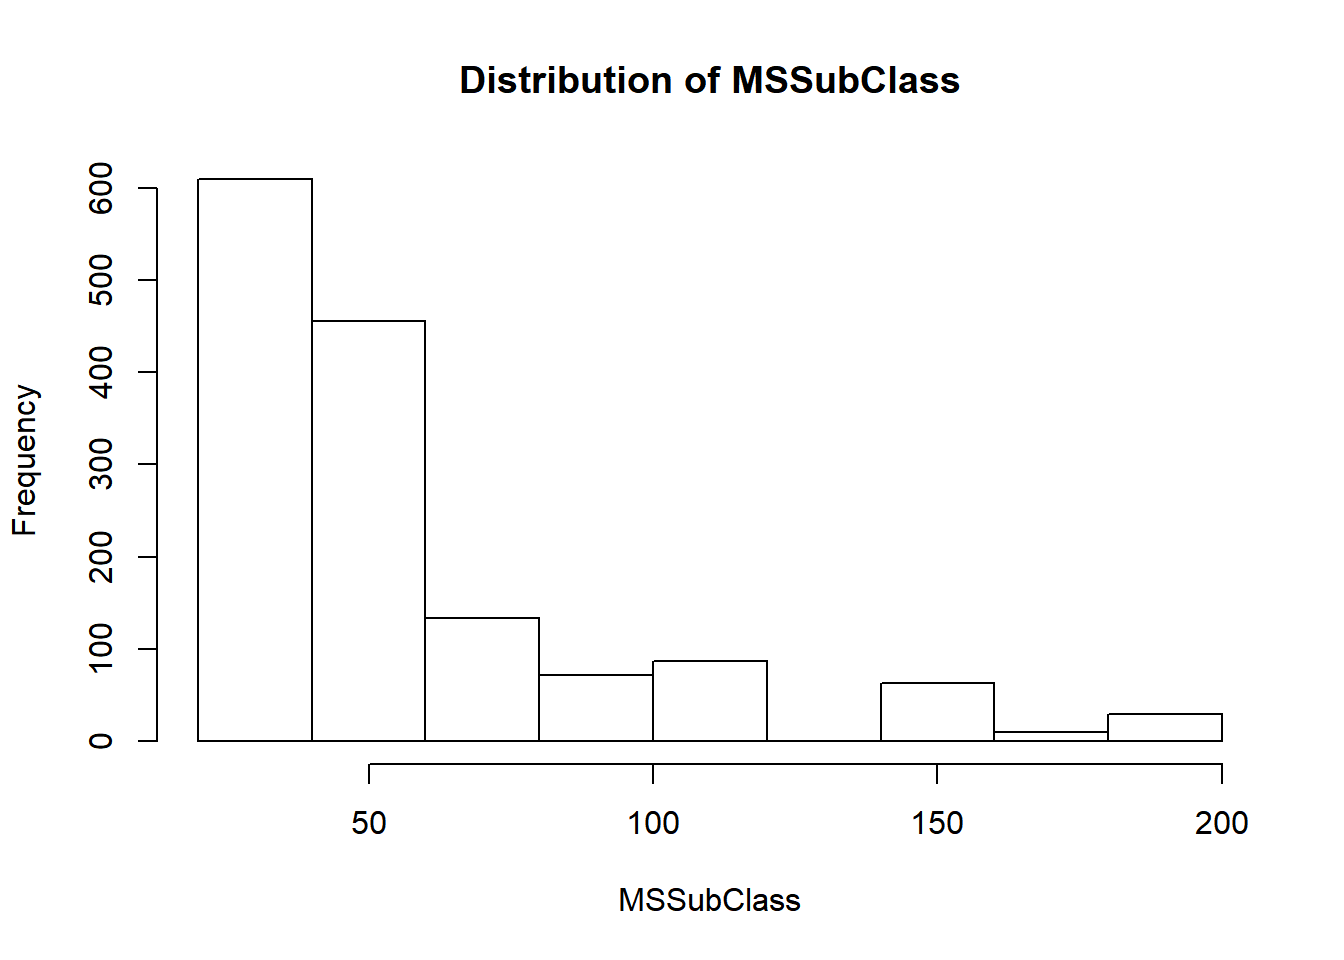
\includegraphics{OOzeren_Final_Exam_files/figure-latex/unnamed-chunk-11-1.pdf}

MSSubClass is left skewed.

\begin{Shaded}
\begin{Highlighting}[]
\KeywordTok{barplot}\NormalTok{(}\KeywordTok{table}\NormalTok{(train}\OperatorTok{$}\NormalTok{MSZoning), }\DataTypeTok{main=}\StringTok{"MS Zoning"}\NormalTok{)}
\end{Highlighting}
\end{Shaded}

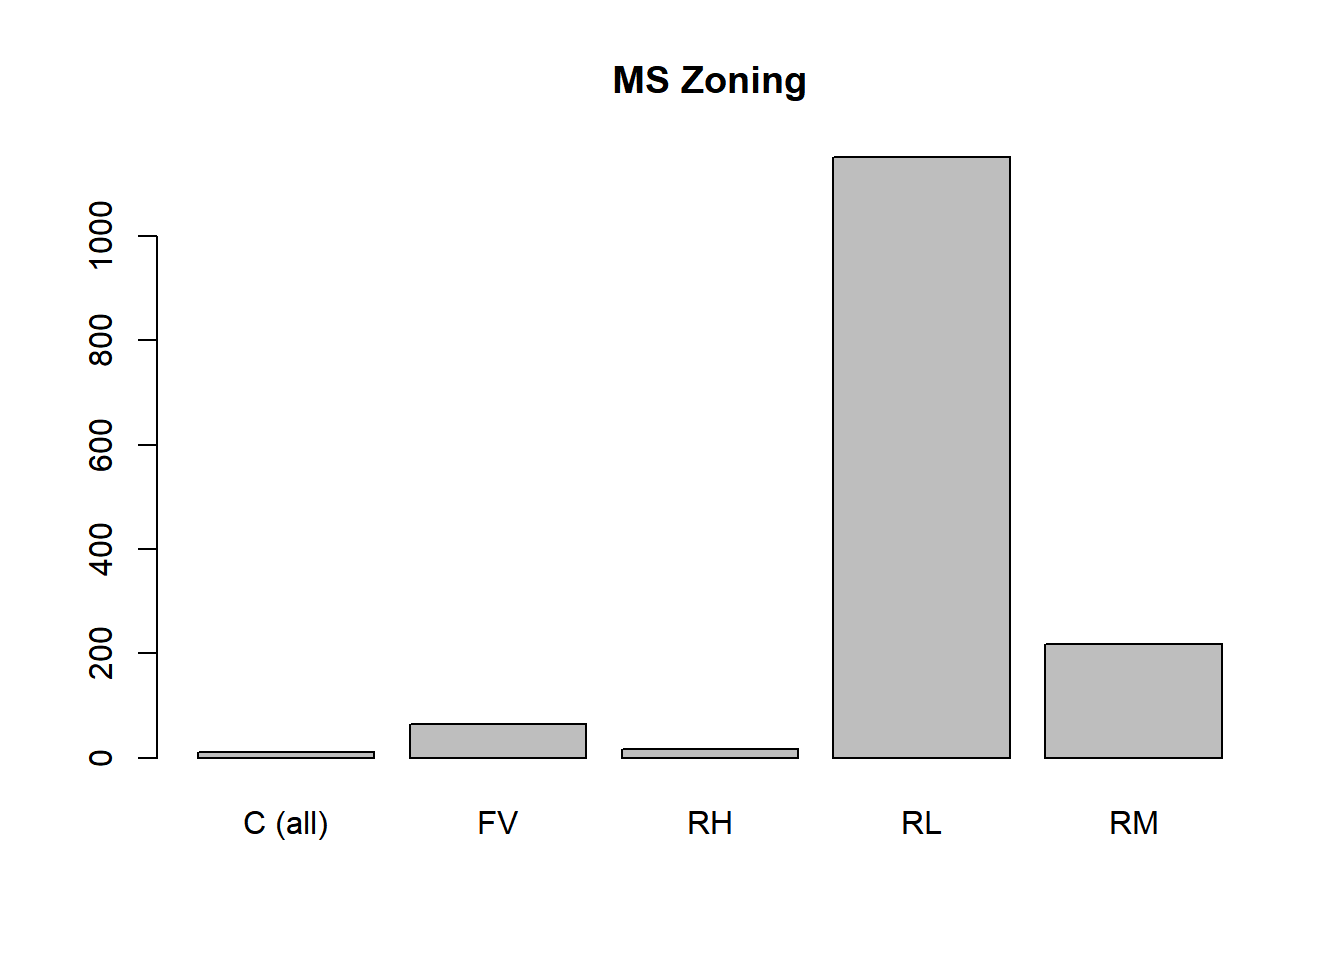
\includegraphics{OOzeren_Final_Exam_files/figure-latex/unnamed-chunk-12-1.pdf}
RL has the highest frequency , C lowest frequency.

\begin{Shaded}
\begin{Highlighting}[]
\KeywordTok{hist}\NormalTok{(train}\OperatorTok{$}\NormalTok{LotFrontage,}\DataTypeTok{main=}\StringTok{"Histogram of Lot Frontage"}\NormalTok{,}\DataTypeTok{xlab=}\StringTok{"LotFrontage"}\NormalTok{)}
\end{Highlighting}
\end{Shaded}

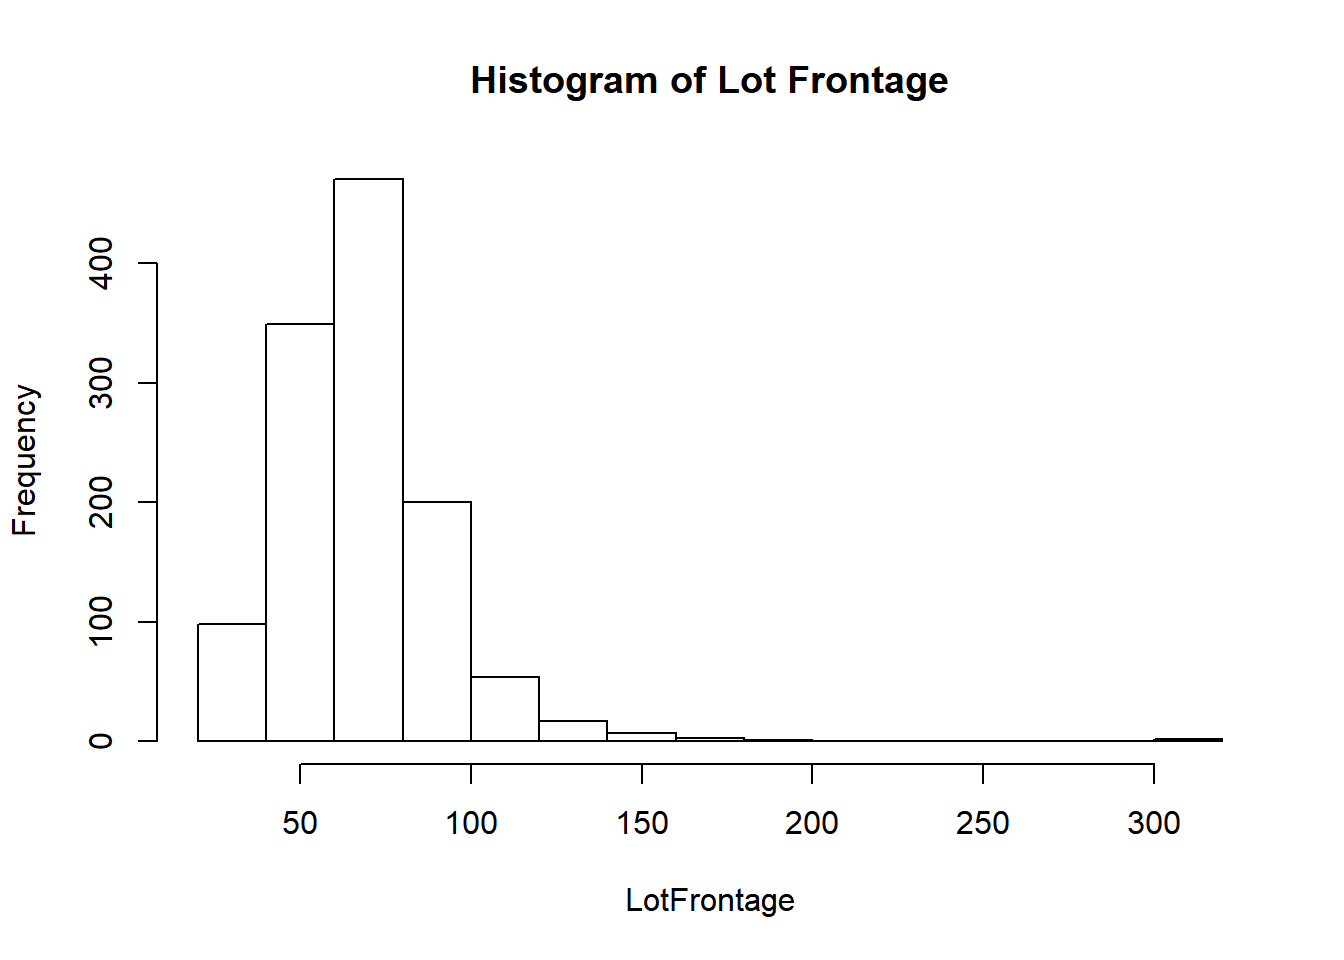
\includegraphics{OOzeren_Final_Exam_files/figure-latex/unnamed-chunk-13-1.pdf}
LotFrontage is left skewed.

\begin{Shaded}
\begin{Highlighting}[]
\KeywordTok{hist}\NormalTok{(train}\OperatorTok{$}\NormalTok{LotArea,}\DataTypeTok{main=}\StringTok{"Distribution of LotArea"}\NormalTok{,}\DataTypeTok{xlab=}\StringTok{"Lot Area"}\NormalTok{)}
\end{Highlighting}
\end{Shaded}

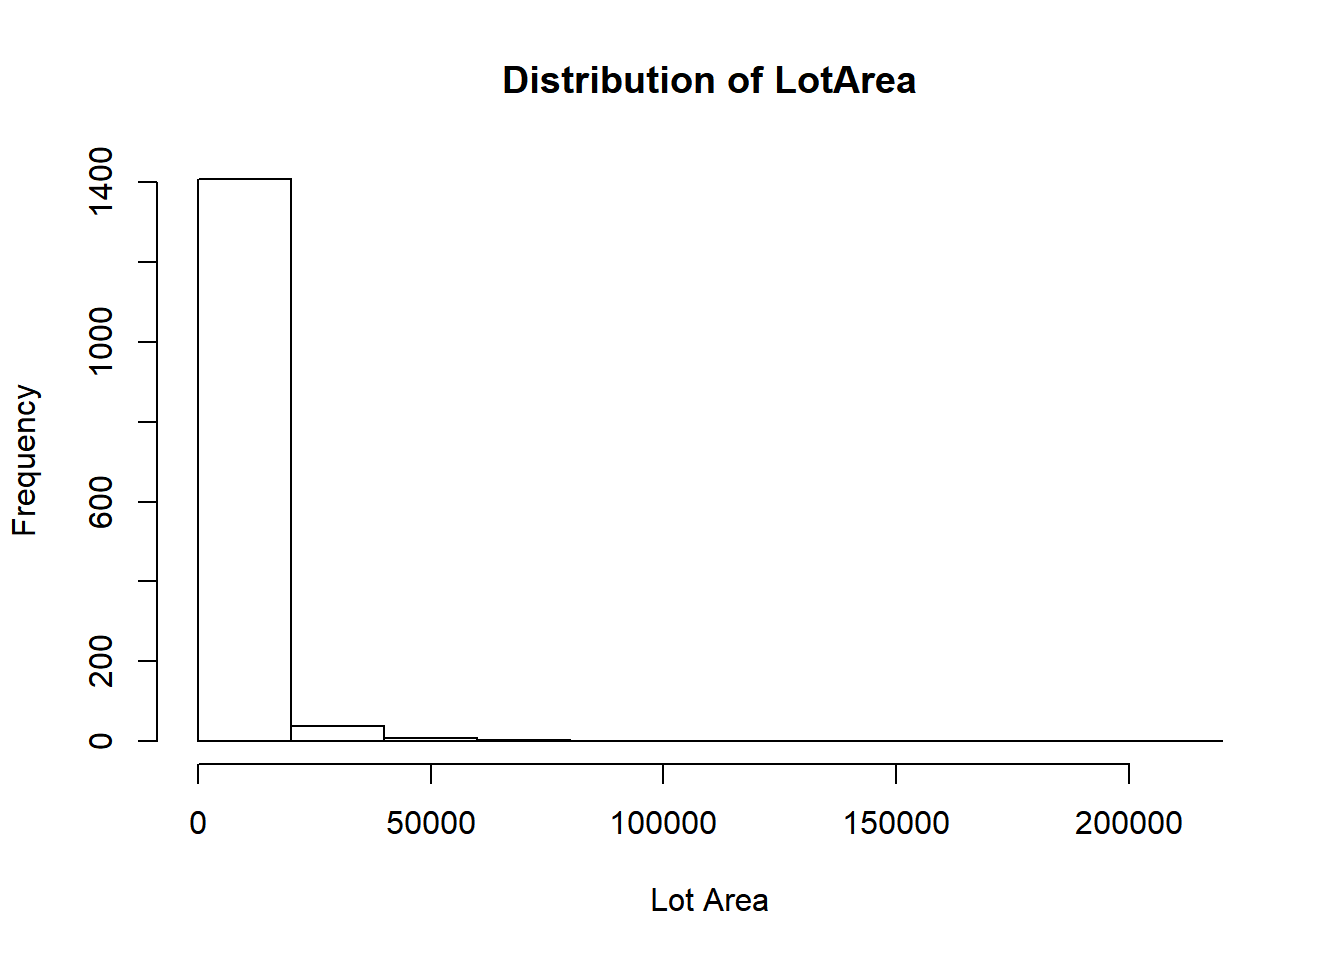
\includegraphics{OOzeren_Final_Exam_files/figure-latex/unnamed-chunk-14-1.pdf}

Lot Area is left skewed with very high small values.

\begin{Shaded}
\begin{Highlighting}[]
\KeywordTok{hist}\NormalTok{(train}\OperatorTok{$}\NormalTok{SalePrice,}\DataTypeTok{main=}\StringTok{"Distribution of Sale Price"}\NormalTok{,}\DataTypeTok{xlab=}\StringTok{"Sale Price"}\NormalTok{)}
\end{Highlighting}
\end{Shaded}

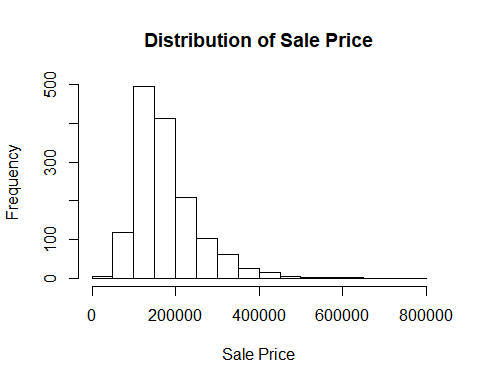
\includegraphics{OOzeren_Final_Exam_files/figure-latex/unnamed-chunk-15-1.pdf}

Sales price is slightly approximately normally distributed. .

\begin{Shaded}
\begin{Highlighting}[]
\KeywordTok{hist}\NormalTok{(train}\OperatorTok{$}\NormalTok{GrLivArea,}\DataTypeTok{main=}\StringTok{"Distribution of Ground Living Area"}\NormalTok{,}\DataTypeTok{xlab=}\StringTok{"Ground Living Area"}\NormalTok{)}
\end{Highlighting}
\end{Shaded}

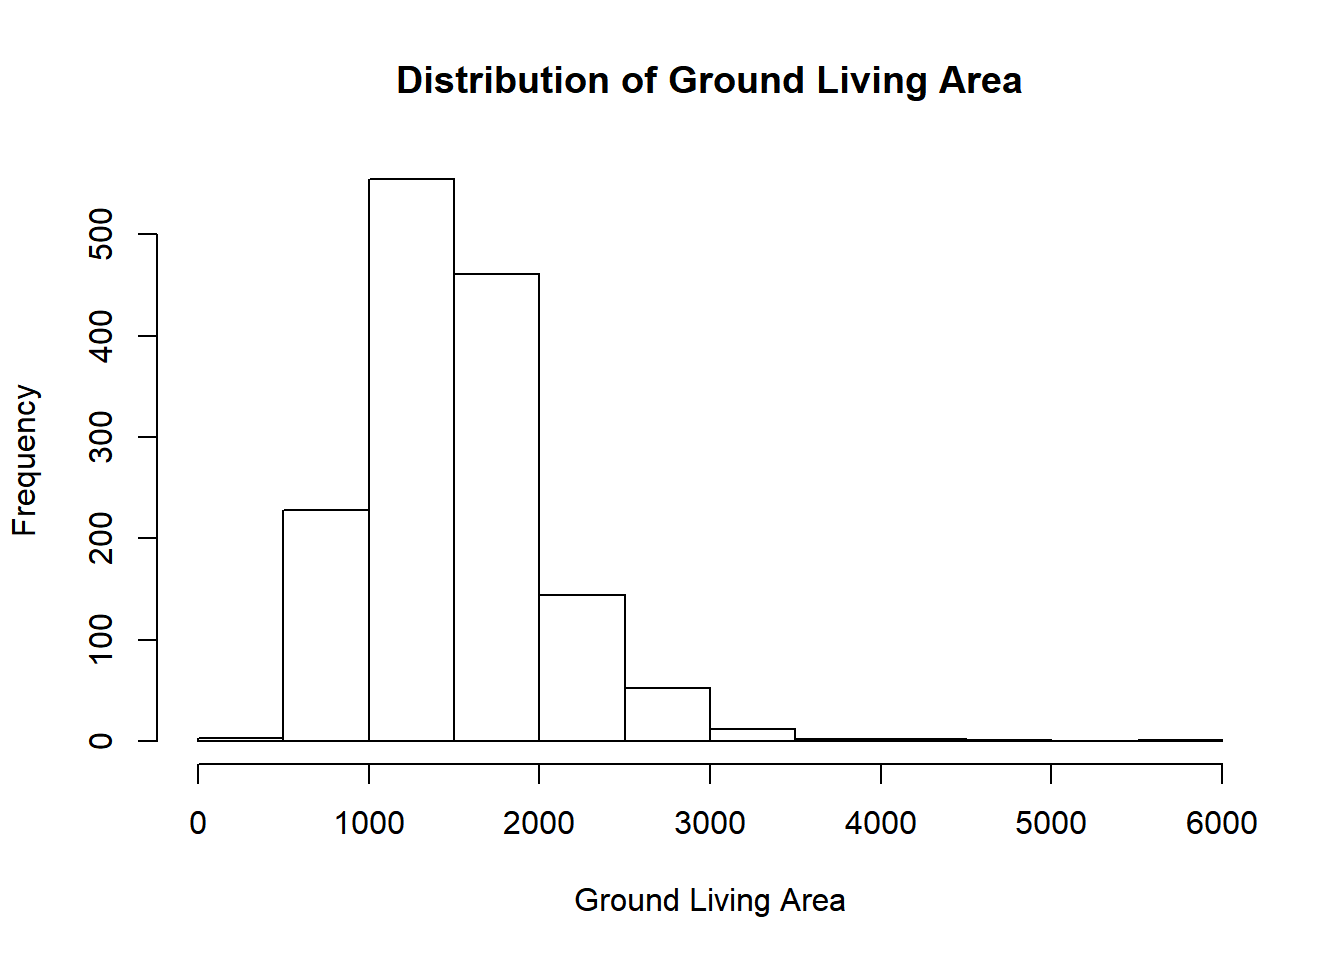
\includegraphics{OOzeren_Final_Exam_files/figure-latex/unnamed-chunk-16-1.pdf}

Ground Living Area is approximately normally distributed.

\textbf{Since the SalePrice column will be the target variable, we'll
start there and look at how it is distributed.}

\begin{Shaded}
\begin{Highlighting}[]
\CommentTok{# Plot SalePrice}
\NormalTok{train }\OperatorTok\StringTok{ }\KeywordTok{ggplot}\NormalTok{(}\KeywordTok{aes}\NormalTok{(}\DataTypeTok{y=}\NormalTok{SalePrice)) }\OperatorTok{+}\StringTok{ }
\StringTok{  }\KeywordTok{geom_boxplot}\NormalTok{(}\DataTypeTok{outlier.color=}\StringTok{"blue"}\NormalTok{, }\DataTypeTok{outlier.alpha =} \FloatTok{0.2}\NormalTok{) }\OperatorTok{+}
\StringTok{  }\KeywordTok{scale_x_discrete}\NormalTok{() }\OperatorTok{+}
\StringTok{  }\KeywordTok{stat_boxplot}\NormalTok{(}\DataTypeTok{geom =}\StringTok{'errorbar'}\NormalTok{,}\DataTypeTok{width=}\NormalTok{.}\DecValTok{3}\NormalTok{) }\OperatorTok{+}
\StringTok{  }\KeywordTok{labs}\NormalTok{(}\DataTypeTok{title=}\StringTok{"Distribution of Sale Price"}\NormalTok{,}
       \DataTypeTok{subtitle=}\StringTok{"Homes"}\NormalTok{, }\DataTypeTok{y=}\StringTok{"Price($)"}\NormalTok{,}
       \DataTypeTok{x=}\StringTok{"Homes"}\NormalTok{) }\OperatorTok{+}\StringTok{ }\KeywordTok{theme_classic}\NormalTok{()}
\end{Highlighting}
\end{Shaded}

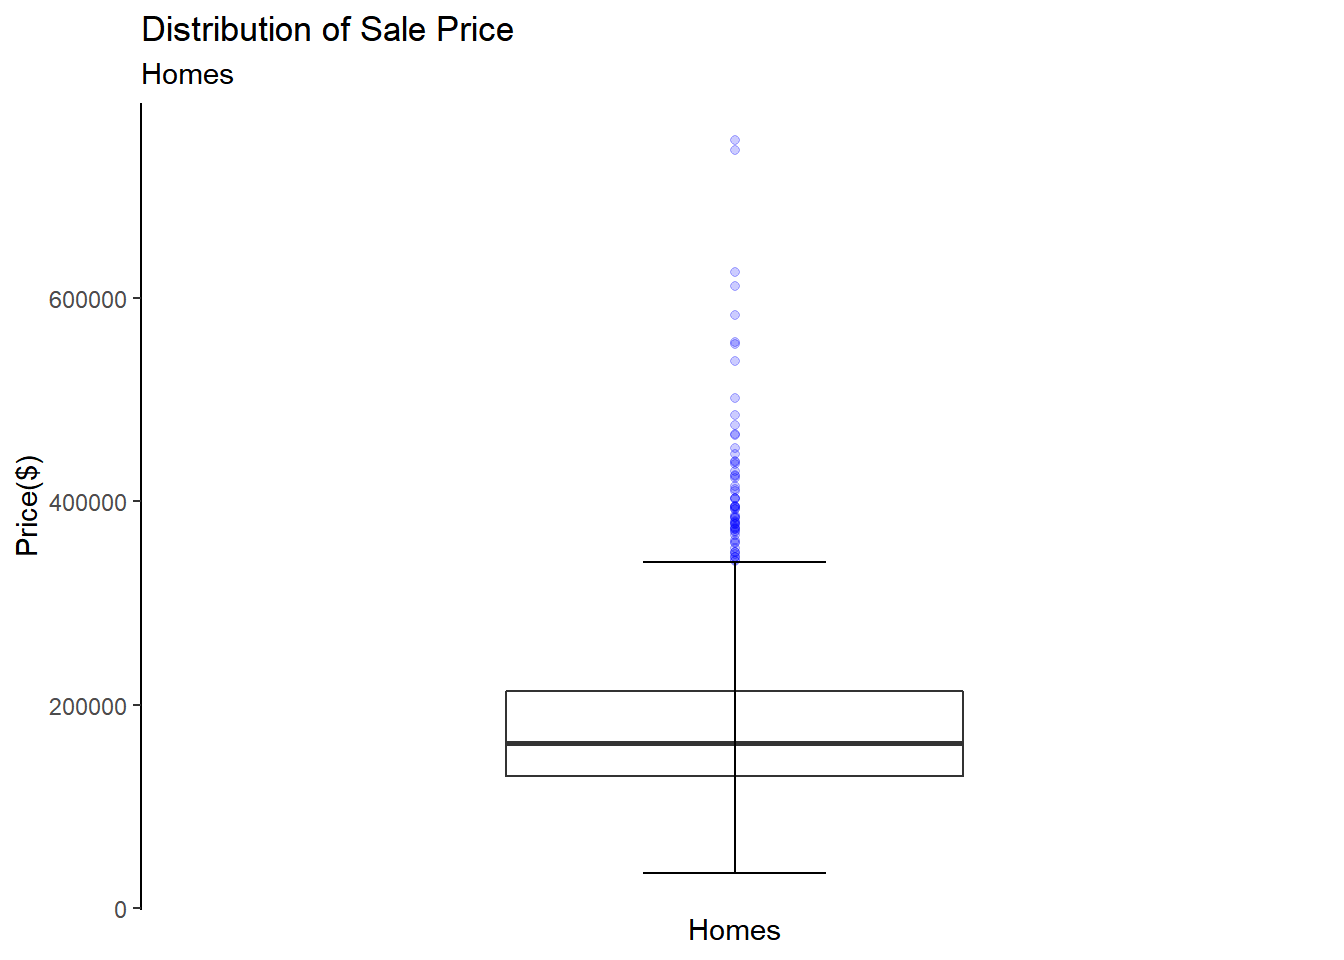
\includegraphics{OOzeren_Final_Exam_files/figure-latex/unnamed-chunk-17-1.pdf}

The Plot above displays that the mean price of houses below \$200K and
they are mostly evenly distributed with some significant outliers above
\$600K range.

\paragraph{ScatterPlot}\label{scatterplot}

\textbf{Scatterplot matrix for
``SalePrice'',``GrLivArea'',``LotFrontage''}

\begin{Shaded}
\begin{Highlighting}[]
\KeywordTok{pairs}\NormalTok{(train[,}\KeywordTok{c}\NormalTok{(}\StringTok{"SalePrice"}\NormalTok{,}\StringTok{"GrLivArea"}\NormalTok{,}\StringTok{"LotFrontage"}\NormalTok{)])}
\end{Highlighting}
\end{Shaded}

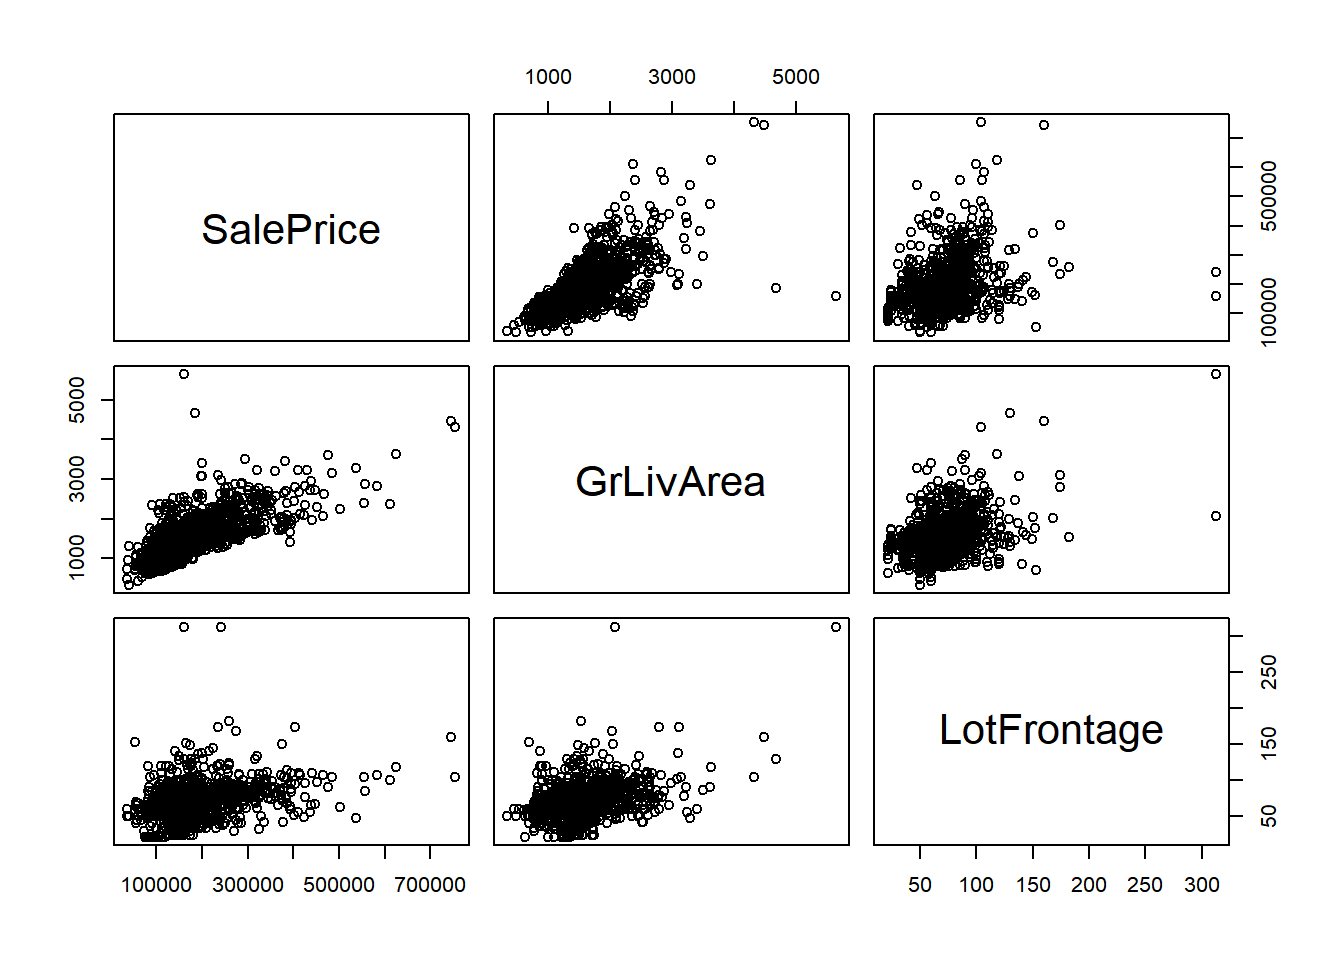
\includegraphics{OOzeren_Final_Exam_files/figure-latex/unnamed-chunk-18-1.pdf}

\textbf{From the scatter plot we can see that GrLiveArea and LotFrontage
are positively correlated with Sale Price.} \textbf{Since Most of the
sale prices are concentrated between 100k and 300k, while the lot sizes
have much less spread.} \textbf{The larger lot sizes do not necessarily
belong to the most expensive properties, which is why we do not see a
stronger correlation.}

\paragraph{Correlation matrix}\label{correlation-matrix}

\begin{Shaded}
\begin{Highlighting}[]
\NormalTok{cormat <-}\StringTok{ }\KeywordTok{cor}\NormalTok{(train[,}\KeywordTok{c}\NormalTok{(}\StringTok{"SalePrice"}\NormalTok{,}\StringTok{"GrLivArea"}\NormalTok{,}\StringTok{"TotalBsmtSF"}\NormalTok{)])}
\NormalTok{cormat}
\end{Highlighting}
\end{Shaded}

\begin{verbatim}
##             SalePrice GrLivArea TotalBsmtSF
## SalePrice   1.0000000 0.7086245   0.6135806
## GrLivArea   0.7086245 1.0000000   0.4548682
## TotalBsmtSF 0.6135806 0.4548682   1.0000000
\end{verbatim}

\begin{Shaded}
\begin{Highlighting}[]
\CommentTok{# Subset of variables}
\NormalTok{train_cor <-}\StringTok{ }\NormalTok{train  }\OperatorTok\StringTok{ }\NormalTok{dplyr}\OperatorTok{::}\KeywordTok{select}\NormalTok{(SalePrice, GrLivArea, TotalBsmtSF)}

\CommentTok{# Compute correlations}
\NormalTok{corr <-}\StringTok{ }\KeywordTok{cor}\NormalTok{(train_cor)}
\KeywordTok{ggcorrplot}\NormalTok{(corr,}\DataTypeTok{lab=}\OtherTok{TRUE}\NormalTok{, }\DataTypeTok{ggtheme =}\NormalTok{ ggplot2}\OperatorTok{::}\NormalTok{theme_classic) }\OperatorTok{+}
\StringTok{  }\KeywordTok{labs}\NormalTok{(}\DataTypeTok{title=}\StringTok{"Correlation"}\NormalTok{,}\DataTypeTok{subtitle=}\StringTok{"All Houses"}\NormalTok{)}
\end{Highlighting}
\end{Shaded}

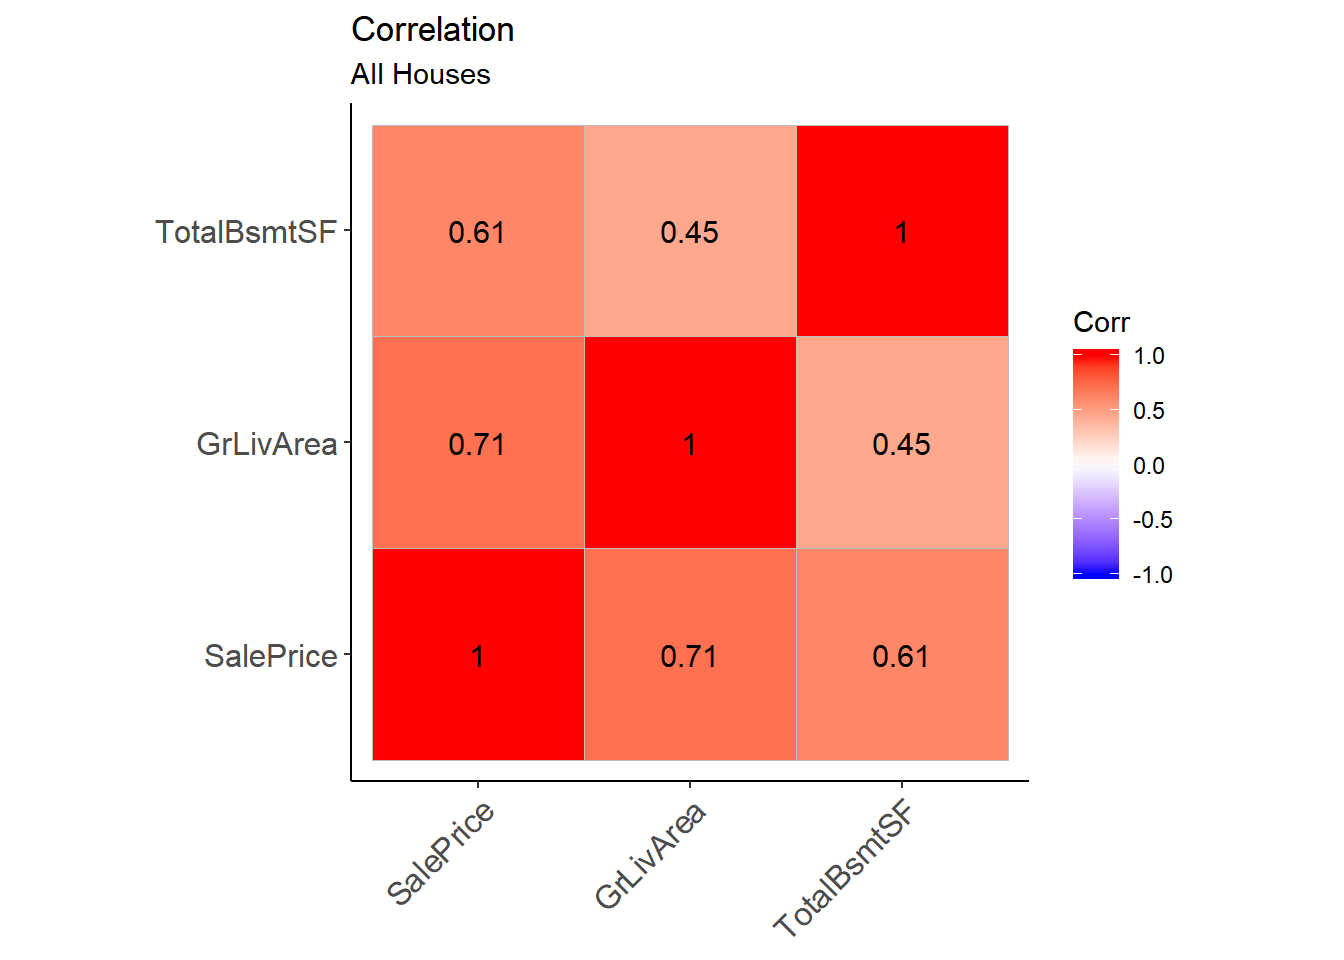
\includegraphics{OOzeren_Final_Exam_files/figure-latex/unnamed-chunk-20-1.pdf}

\textbf{The graph above displays that Sale Price shows strong positive
correlation with ``GrLivArea''" and moderate correlation with
TotalBsmTSF.} \textbf{In Addition,``GrLivArea''" shows Strong positive
correlation with SalePrice and weak positive correlation with
``TotalBsmSF'' and also} \textbf{``TotalBsmSF''" shows moderate positive
correlation with SalePrice and weak positive correlation with
``GrLivArea''.}

\paragraph{Hypothesis and 80\% confidence
interval}\label{hypothesis-and-80-confidence-interval}

Test the hypotheses that the correlations between each pairwise set of
variables is 0 and provide an 80\% confidence interval.Discuss the
meaning of your analysis. Would you be worried about familywise error?
Why or why not?

Null (Ho) Hypothesis: The correlation between GrLivArea and SalePrice is
0 Alternative(H1) Hypothesis: The correlation between GrLivArea and
SalePrice is other than 0

\begin{Shaded}
\begin{Highlighting}[]
\KeywordTok{cor.test}\NormalTok{(train}\OperatorTok{$}\NormalTok{GrLivArea, train}\OperatorTok{$}\NormalTok{TotalBsmtSF, }\DataTypeTok{conf.level =} \FloatTok{0.8}\NormalTok{)}
\end{Highlighting}
\end{Shaded}

\begin{verbatim}
## 
##  Pearson's product-moment correlation
## 
## data:  train$GrLivArea and train$TotalBsmtSF
## t = 19.503, df = 1458, p-value < 0.00000000000000022
## alternative hypothesis: true correlation is not equal to 0
## 80 percent confidence interval:
##  0.4278380 0.4810855
## sample estimates:
##       cor 
## 0.4548682
\end{verbatim}

Since the the p value of the test is less than 0.05 at 5\% level of
significance we reject the null hypothesis and conclude that the
correlation between \textbf{GrLivArea} and \textbf{TotalBsmtSF} is other
than 0.

80 percent confidence interval of the test is 0.4327076 0.4879552

\begin{Shaded}
\begin{Highlighting}[]
\KeywordTok{cor.test}\NormalTok{(train}\OperatorTok{$}\NormalTok{SalePrice, train}\OperatorTok{$}\NormalTok{TotalBsmtSF, }\DataTypeTok{conf.level =} \FloatTok{0.8}\NormalTok{)}
\end{Highlighting}
\end{Shaded}

\begin{verbatim}
## 
##  Pearson's product-moment correlation
## 
## data:  train$SalePrice and train$TotalBsmtSF
## t = 29.671, df = 1458, p-value < 0.00000000000000022
## alternative hypothesis: true correlation is not equal to 0
## 80 percent confidence interval:
##  0.5922142 0.6340846
## sample estimates:
##       cor 
## 0.6135806
\end{verbatim}

Since the the p value of the test is less than 0.05 at 5\% level of
significance we reject the null hypothesis and conclude that the
correlation between \textbf{SalePrice} and \textbf{TotalBsmtSF} is other
than 0.

80 percent confidence interval of the test is 0.5922142 0.6340846

\begin{Shaded}
\begin{Highlighting}[]
\KeywordTok{cor.test}\NormalTok{(train}\OperatorTok{$}\NormalTok{SalePrice, train}\OperatorTok{$}\NormalTok{GrLivArea, }\DataTypeTok{conf.level =} \FloatTok{0.8}\NormalTok{)}
\end{Highlighting}
\end{Shaded}

\begin{verbatim}
## 
##  Pearson's product-moment correlation
## 
## data:  train$SalePrice and train$GrLivArea
## t = 38.348, df = 1458, p-value < 0.00000000000000022
## alternative hypothesis: true correlation is not equal to 0
## 80 percent confidence interval:
##  0.6915087 0.7249450
## sample estimates:
##       cor 
## 0.7086245
\end{verbatim}

Since the the p value of the test is less than 0.05 at 5\% level of
significance we reject the null hypothesis and conclude that the
correlation between \textbf{SalePrice} and \textbf{GrLivArea} is other
than 0.

80 percent confidence interval of the test is 0.6915087 0.7249450

\paragraph{Familywise Error}\label{familywise-error}

type I error is the rejection of a true null hypothesis (also known as a
``false positive'' finding or conclusion)

\begin{Shaded}
\begin{Highlighting}[]
\NormalTok{FWE <-}\StringTok{ }\DecValTok{1} \OperatorTok{-}\StringTok{ }\NormalTok{(}\DecValTok{1} \OperatorTok{-}\StringTok{ }\NormalTok{.}\DecValTok{05}\NormalTok{)}\OperatorTok{^}\DecValTok{2} 
\NormalTok{FWE}
\end{Highlighting}
\end{Shaded}

\begin{verbatim}
## [1] 0.0975
\end{verbatim}

There is a 9.75\% chance of type 1 error. Since the chance is low I will
not be worried for family wise error .

\subsubsection{5 points. Linear Algebra and
Correlation.}\label{points.-linear-algebra-and-correlation.}

Invert your correlation matrix from above. (This is known as the
precision matrix and contains variance inflation factors on the
diagonal.) Multiply the correlation matrix by the precision matrix, and
then multiply the precision matrix by the correlation matrix. Conduct LU
decomposition on the matrix.

Invert your correlation matrix.This is known as the precision matrix and
contains variance inflation factors on the diagonal.

\begin{Shaded}
\begin{Highlighting}[]
\CommentTok{# find inverse}
\NormalTok{precision_mat <-}\StringTok{ }\KeywordTok{solve}\NormalTok{(cormat)}
\end{Highlighting}
\end{Shaded}

Multiply the correlation matrix by the precision matrix, and then
multiply the precision matrix by the correlation matrix.

\begin{Shaded}
\begin{Highlighting}[]
\CommentTok{# Multiply the correlation matrix by the precision matrix}
\NormalTok{cor_prec <-}\StringTok{ }\NormalTok{cormat }\OperatorTok\StringTok{ }\NormalTok{precision_mat}
\NormalTok{cor_prec}
\end{Highlighting}
\end{Shaded}

\begin{verbatim}
##                             SalePrice                  GrLivArea
## SalePrice   1.00000000000000022204460 -0.00000000000000002081668
## GrLivArea   0.00000000000000005551115  1.00000000000000000000000
## TotalBsmtSF 0.00000000000000000000000  0.00000000000000005551115
##                          TotalBsmtSF
## SalePrice   0.0000000000000000000000
## GrLivArea   0.0000000000000001110223
## TotalBsmtSF 1.0000000000000000000000
\end{verbatim}

\begin{Shaded}
\begin{Highlighting}[]
\CommentTok{#  multiply the precision matrix by the correlation matrix}
\NormalTok{prec_cor <-}\StringTok{   }\NormalTok{precision_mat }\OperatorTok\StringTok{ }\NormalTok{cormat}
\NormalTok{prec_cor}
\end{Highlighting}
\end{Shaded}

\begin{verbatim}
##                            SalePrice                 GrLivArea
## SalePrice   0.9999999999999997779554 -0.0000000000000001665335
## GrLivArea   0.0000000000000002012279  1.0000000000000004440892
## TotalBsmtSF 0.0000000000000000000000  0.0000000000000001110223
##                           TotalBsmtSF
## SalePrice   -0.0000000000000001110223
## GrLivArea    0.0000000000000001665335
## TotalBsmtSF  1.0000000000000000000000
\end{verbatim}

\begin{Shaded}
\begin{Highlighting}[]
\CommentTok{# LU Decomposistion}
\KeywordTok{library}\NormalTok{(pracma)}
\end{Highlighting}
\end{Shaded}

\begin{verbatim}
## Warning: package 'pracma' was built under R version 3.5.3
\end{verbatim}

\begin{verbatim}
## 
## Attaching package: 'pracma'
\end{verbatim}

\begin{verbatim}
## The following object is masked from 'package:purrr':
## 
##     cross
\end{verbatim}

\begin{Shaded}
\begin{Highlighting}[]
\KeywordTok{lu}\NormalTok{(cormat)}
\end{Highlighting}
\end{Shaded}

\begin{verbatim}
## $L
##             SalePrice  GrLivArea TotalBsmtSF
## SalePrice   1.0000000 0.00000000           0
## GrLivArea   0.7086245 1.00000000           0
## TotalBsmtSF 0.6135806 0.04031325           1
## 
## $U
##             SalePrice GrLivArea TotalBsmtSF
## SalePrice           1 0.7086245   0.6135806
## GrLivArea           0 0.4978513   0.0200700
## TotalBsmtSF         0 0.0000000   0.6227098
\end{verbatim}

\subsubsection{Calculus-Based Probability \&
Statistics.}\label{calculus-based-probability-statistics.}

Many times, it makes sense to fit a closed form distribution to data.
Select a variable in the Kaggle.com training dataset that is skewed to
the right, shift it so that the minimum value is absolutely above zero
if necessary. Then load the MASS package and run fitdistr to fit an
exponential probability density function. (See
\url{https://stat.ethz.ch/R-manual/R-devel/library/MASS/html/fitdistr.html}
). Find the optimal value of ??? for this distribution, and then take
1000 samples from this exponential distribution using this value (e.g.,
rexp(1000, ???)). Plot a histogram and compare it with a histogram of
your original variable. Using the exponential pdf, find the 5th and 95th
percentiles using the cumulative distribution function (CDF). Also
generate a 95\% confidence interval from the empirical data, assuming
normality. Finally, provide the empirical 5th percentile and 95th
percentile of the data. Discuss.

\begin{Shaded}
\begin{Highlighting}[]
\KeywordTok{library}\NormalTok{(MASS)}
\end{Highlighting}
\end{Shaded}

\begin{verbatim}
## Warning: package 'MASS' was built under R version 3.5.3
\end{verbatim}

\begin{verbatim}
## 
## Attaching package: 'MASS'
\end{verbatim}

\begin{verbatim}
## The following object is masked from 'package:dplyr':
## 
##     select
\end{verbatim}

\paragraph{Univariate distribution of
LotArea}\label{univariate-distribution-of-lotarea}

\begin{Shaded}
\begin{Highlighting}[]
\NormalTok{(expdf <-}\StringTok{ }\KeywordTok{fitdistr}\NormalTok{(train}\OperatorTok{$}\NormalTok{LotArea, }\StringTok{"exponential"}\NormalTok{))}
\end{Highlighting}
\end{Shaded}

\begin{verbatim}
##         rate     
##   0.000095085704 
##  (0.000002488507)
\end{verbatim}

\begin{Shaded}
\begin{Highlighting}[]
\CommentTok{# get value of lambda from exponential distribution}
\NormalTok{lambda <-}\StringTok{ }\NormalTok{expdf}\OperatorTok{$}\NormalTok{estimate}

\CommentTok{# expected value of lambda}
\NormalTok{rate <-}\StringTok{ }\DecValTok{1} \OperatorTok{/}\StringTok{ }\NormalTok{lambda}
\NormalTok{rate}
\end{Highlighting}
\end{Shaded}

\begin{verbatim}
##     rate 
## 10516.83
\end{verbatim}

\textbf{Then, take 1000 samples from this exponential distribution using
this value. (e.g., rexp(1000, some\_val))((()))}

\begin{Shaded}
\begin{Highlighting}[]
\CommentTok{# 1000 samples from exponential distribution using lambda}
\NormalTok{expdf_samp <-}\StringTok{ }\KeywordTok{rexp}\NormalTok{(}\DecValTok{1000}\NormalTok{, lambda)}
\end{Highlighting}
\end{Shaded}

\textbf{Plot a histogram and compare it with a histogram of your
original variable.}

\begin{Shaded}
\begin{Highlighting}[]
\CommentTok{# Actual vs simulated distribution}
\KeywordTok{hist}\NormalTok{(train}\OperatorTok{$}\NormalTok{LotArea, }\DataTypeTok{breaks=}\DecValTok{50}\NormalTok{, }\DataTypeTok{prob=}\OtherTok{TRUE}\NormalTok{,}\DataTypeTok{col=}\StringTok{"royalblue"}\NormalTok{, }\DataTypeTok{xlab=}\StringTok{"Actual Lot Area"}\NormalTok{,}
     \DataTypeTok{main=}\StringTok{"Lot Area Distribution"}\NormalTok{)}
\end{Highlighting}
\end{Shaded}

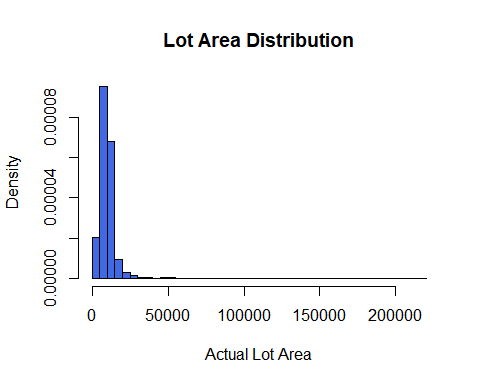
\includegraphics{OOzeren_Final_Exam_files/figure-latex/unnamed-chunk-31-1.pdf}

\begin{Shaded}
\begin{Highlighting}[]
\KeywordTok{hist}\NormalTok{(expdf_samp, }\DataTypeTok{breaks=}\DecValTok{50}\NormalTok{, }\DataTypeTok{prob=}\OtherTok{TRUE}\NormalTok{,}\DataTypeTok{col=}\StringTok{"royalblue"}\NormalTok{, }\DataTypeTok{xlab=}\StringTok{"Generated(Estimated) Data"}\NormalTok{,}
     \DataTypeTok{main=}\StringTok{"Generated(Estimated) Data's Distribution"}\NormalTok{)}
\end{Highlighting}
\end{Shaded}

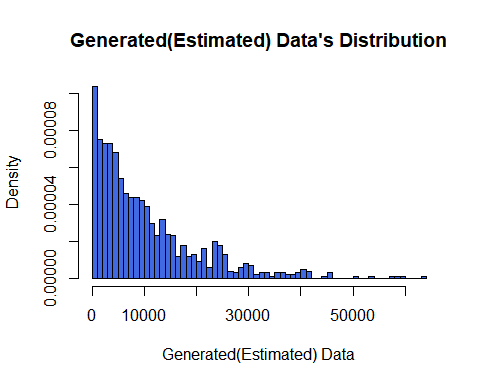
\includegraphics{OOzeren_Final_Exam_files/figure-latex/unnamed-chunk-31-2.pdf}

As we can see plots here that our Lot Area approximately fits a
exponential distribution. The fit does not do good job here.Let's look
at the summary table to understand the details

\begin{Shaded}
\begin{Highlighting}[]
\CommentTok{# Actuals Data summary Table}
\KeywordTok{summary}\NormalTok{(expdf_samp)}
\end{Highlighting}
\end{Shaded}

\begin{verbatim}
##     Min.  1st Qu.   Median     Mean  3rd Qu.     Max. 
##     0.79  3160.25  7632.81 10656.20 15123.29 64761.28
\end{verbatim}

\begin{Shaded}
\begin{Highlighting}[]
\CommentTok{# Generated Data summary Table}
\KeywordTok{summary}\NormalTok{(train}\OperatorTok{$}\NormalTok{LotArea)}
\end{Highlighting}
\end{Shaded}

\begin{verbatim}
##    Min. 1st Qu.  Median    Mean 3rd Qu.    Max. 
##    1300    7554    9478   10517   11602  215245
\end{verbatim}

\subsubsection{CDF}\label{cdf}

5th and 95th percentiles using the cumulative distribution function
(CDF)

\begin{Shaded}
\begin{Highlighting}[]
\NormalTok{cdf <-}\StringTok{ }\KeywordTok{ecdf}\NormalTok{(expdf_samp)}
\NormalTok{expdf_samp[}\KeywordTok{cdf}\NormalTok{(expdf_samp)}\OperatorTok{==}\FloatTok{0.05}\NormalTok{]}
\end{Highlighting}
\end{Shaded}

\begin{verbatim}
## [1] 516.3167
\end{verbatim}


\end{document}
